\documentclass[handout]{beamer}

\usepackage{Vor2018glærur}

\title{Tölvunarfræði 2}
\subtitle{Vika 7}

\begin{document}

\begin{frame}
	\titlepage
\end{frame}

\section{Miðmisseriskönnun}

\begin{frame}{Miðmisseriskönnun}
	\begin{center}
		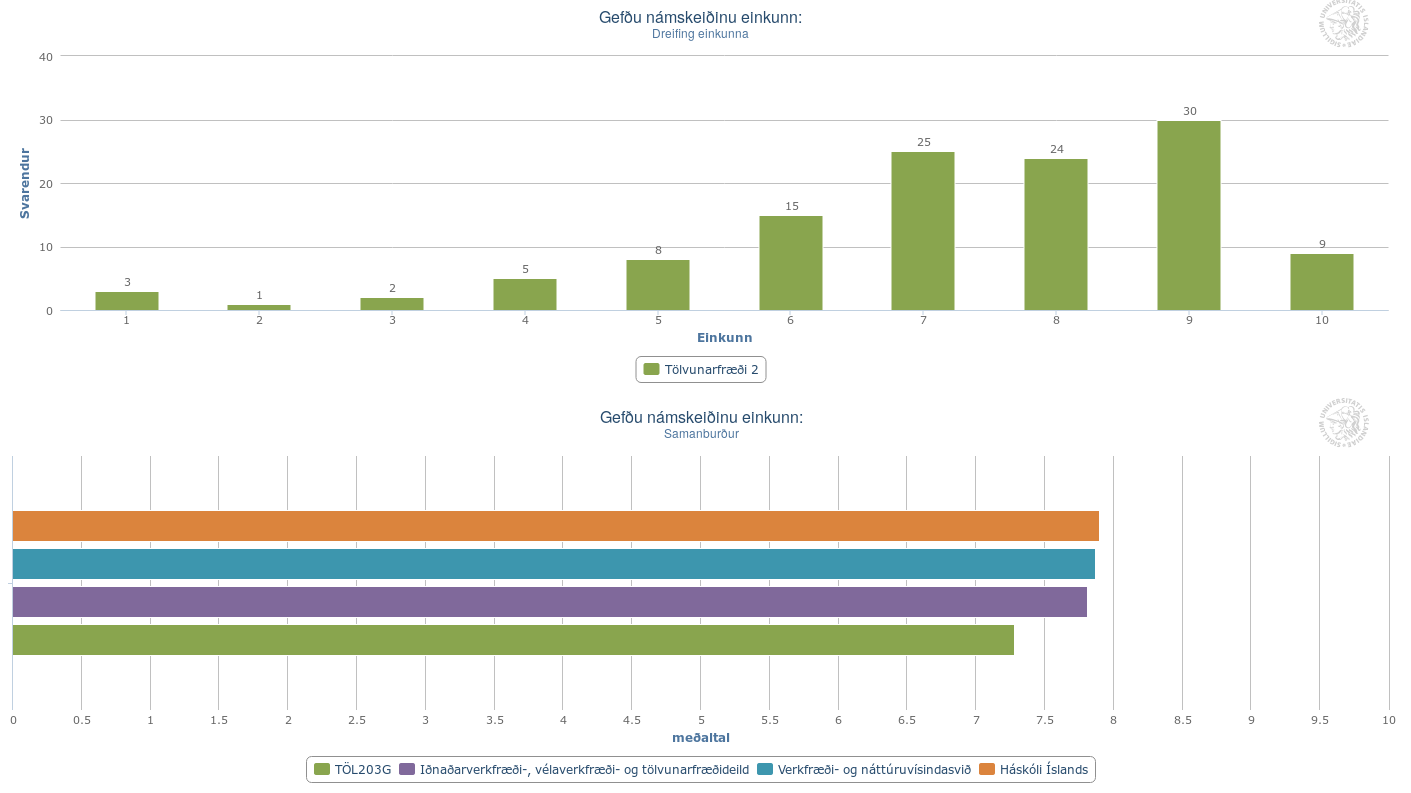
\includegraphics[width=\textwidth]{midmisseriskonnun-2018}
	\end{center}
\end{frame}

\begin{frame}{Atriði sem komu fram}
	\begin{itemize}
		\item Meðaleinkunn 7.28, 50.00\% þáttakka
		\item (Meðaleinkunn 6.1, 45\% þátttaka í fyrra)
		\item Gott:
		      \begin{itemize}
			      \item Fyrirlestrarnir og upptökur
			      \item Piazza
			      \item Framsetning skilaverkefna
		      \end{itemize}
		\item Verra:
		      \begin{itemize}
			      \item Salurinn er ekki nógu góður (!!!)
			      \item Erfið heimaverkefni
			      \item Mikið stökk úr tölvunarfræði 1
			      \item Vantar fleiri dæmi til æfingar
		      \end{itemize}
	\end{itemize}
\end{frame}

\section{Quicksort}

\begin{frame}{Quicksort}
	\begin{itemize}
		\item Quicksort er skilvirkt og mikið notað röðunarreiknirit
		      \begin{itemize}
			      \item Hefur verið gríðarlega mikið rannsakað síðan þá
			      \item Kostir og gallar reikniritsins eru vel þekktir
			      \item Meðal rannsakenda: Robert Sedgewick
		      \end{itemize}
		\item Quicksort fundið upp af Tony Hoare 1960
		      \begin{itemize}
			      \item Fann það upp við nám í rússlandi, til að raða orðum
			      \item Hoare er líka þekktur fyrir framlag til formlegra forritunaraðferða og ALGOL forritunarmálsins
		      \end{itemize}
	\end{itemize}
\end{frame}

\begin{frame}{Lýsing}
	\begin{itemize}
		\item Lýsing á quicksort:
		      \begin{enumerate}
			      \item Veljum safn til að raða og eitthvert stak innan þess til að þjóna sem vendistak \eng{pivot}
			      \item Skiptum upp \eng{partition} safninu og endurröðum svo að vendistakið sé á réttum stað, engin stök stærri en vendistakið séu í vinstri hluta þess og engin stök minni en vendistakið séu í hægri hluta þess
			      \item Notum quicksort endurkvæmt á hvorn hluta fyrir sig
		      \end{enumerate}
	\end{itemize}
\end{frame}

\begin{frame}{Deila og drottna}
	\begin{center}
		Quicksort og ofansækin sameiningarröðun eru dæmi um ``deila og drottna'' \eng{divide and conquer}) reiknirit
	\end{center}
	\begin{columns}
		\column{0.5\textwidth}
		Sameiningarröðun:
		\begin{itemize}
			\item[] \textbf{Divide:} Skiptum fylkinu í tvö jafn stór undirfylki
			\item[] \textbf{Conquer:} Notum sameiningarröðun á undirfylkin þar til þau eru af lengd 1 og þ.a.l. röðuð
			\item[] \textbf{Combine:} Sameinum röðuðu undirfylkin
		\end{itemize}
		\column{0.5\textwidth}
		Quicksort:
		\begin{itemize}
			\item[] \textbf{Divide:} Veljum vendistak, skiptum fylkinu í tvö undirfylki þar sem vinstra er minna en vendistak og hægra er stærra en vendistak
			\item[] \textbf{Conquer:} Notum quicksort á undirfylkin
			\item[] \textbf{Combine:} Óþarft
		\end{itemize}
	\end{columns}
\end{frame}

\headonly

\begin{frame}[fragile]{Quicksort}
	\vspace{0.5cm}
	\begin{minted}[frame=lines, fontsize=\small]{java}
public static void sort(Comparable[] a) {
    StdRandom.shuffle(a);
    // Eliminate dependence on input.
    sort(a, 0, a.length - 1);
}

private static void sort(Comparable[] a, int lo, int hi) {
    if (hi <= lo) return;
    int j = partition(a, lo, hi); // Partition (see page 291).
    sort(a, lo, j - 1);
    // Sort left part a[lo .. j-1].
    sort(a, j + 1, hi);
    // Sort right part a[j+1 .. hi].
}
    \end{minted}
	\begin{center}
		Algorithms, 4th edition, bls. 289
	\end{center}
\end{frame}

\begin{frame}[fragile]{Partition aðferðin}
	\vspace{0.5cm}
	\begin{minted}[frame=lines, fontsize=\small]{java}
private static int partition(Comparable[] a, int lo, int hi) { 
    // Partition into a[lo..i-1], a[i], a[i+1..hi].
    int i = lo, j = hi + 1; // left and right scan indices
    Comparable v = a[lo]; // partitioning item
    while (true) {
        while (less(a[++i], v)) if (i == hi) break;
        while (less(v, a[--j])) if (j == lo) break;
        if (i >= j) break;
        exch(a, i, j);
    }
    exch(a, lo, j);
    // Put v = a[j] into position
    return j; // with a[lo..j-1] <= a[j] <= a[j+1..hi].
}
    \end{minted}
	\begin{center}
		Algorithms, 4th edition, bls. 291
	\end{center}
\end{frame}

\headandfoot

\begin{frame}{Skilvirkni}
	\begin{itemize}
		\item Besta mögulega tilfelli quicksort - hvert fallskall myndar helmingaskiptingu á safninu
		      \begin{itemize}
			      \item Besti samanburðarfjölda má lýsa með $C_N = 2C_{N/2} + N$, svo $C_N \sim N \log N$
		      \end{itemize}
		\item Ástæða fyrir raunverulegri skilvirkni - meðaltilfellið er litlu verra en það besta
		      \begin{itemize}
			      \item Ekki nema 39\% fleiri samanburðir í ``meðaltilfellinu''
			      \item Má sanna með tölfræðilegum aðferðum
		      \end{itemize}
		\item Í versta tilfellinu - öll stökin lenda á sömu hlið við vendistakið
		      \begin{itemize}
			      \item $\sim \frac{N^2}{2}$ samanburðir, gríðarlega ólíklegt eftir slembiröðun
		      \end{itemize}
		\item Oft betra en sameiningarröðun vegna fárra skiptinga og eiginleika raunverulegra örgjörva
	\end{itemize}
\end{frame}

\begin{frame}{Endurbætur}
	\begin{itemize}
		\item Hægt er að fá meiri hraða úr quicksort með smábreytingum frá \texttt{Quick.java}
		      \begin{itemize}
			      \item Skipta yfir í innsetningarröðun á smáfylkjum
			      \item Meðhöndla jafn stór stök sérstaklega (3-way partitioning)
			      \item Gott val á vendistaki - t.d. Median-of-3
		      \end{itemize}
	\end{itemize}
\end{frame}

\imageslide{AlgsSlides/sort-comparison}

\section{Forgangsbiðraðir}

\begin{frame}{Forgangsbiðröð}
	\begin{itemize}
		\item Forgangsbiðröð (e. \emph{priority queue}) er hugræn gagnagerð
		\item Almennari gagnagerð en hlaðar og biðraðir, sem við höfum séð áður
		      \begin{itemize}
			      \item Í hlaða: Eyðing framkvæmd á því staki sem styst hefur verið á hlaðanum
			      \item Í biðröð: Eyðing framkvæmd á því staki sem lengst hefur verið í biðröðinni
			      \item Í forgangsbiðröð: Eyðing framkvæmd á því staki sem hefur hæsta ``lykilinn''
			  \end{itemize}
		\item Athugum: Getum látið lykil staks vera eitthvað annað en gildi þess 
	\end{itemize}
\end{frame}

\begin{frame}{API}
	Möguleg skil fyrir forgangsbiðröð:
	\begin{center}
		\begin{tabularx}{\textwidth}{rlX}
			\toprule
			\multicolumn{3}{c}{\texttt{public class MaxPQ<Key extends Comparable<Key>>}}                \\
			\midrule
			-                & \texttt{MaxPQ()}       & Smiður, býr til tóma forgangsbiðröð             \\
			\texttt{void}    & \texttt{insert(Key v)} & Bæta stakinu \texttt{key} við f-biðröðina       \\
			\texttt{Key}     & \texttt{max()}         & Skila stærsta stakinu í biðröðinni              \\
			\texttt{Key}     & \texttt{delMax()}      & Fjarlægja og skila stærsta stakinu í biðröðinni \\
			\texttt{boolean} & \texttt{isEmpty()}     & Er forgangsbiðröðin tóm?                        \\
			\texttt{int}     & \texttt{size()}        & Fjöldi hluta í forgangsbiðröðinni               \\
			\bottomrule
		\end{tabularx}
	\end{center}
	Aths: Gætum allt eins skilgreint ``minimum priority queue''. \texttt{Key} þarf að vera samanburðarhæfur.
\end{frame}

\begin{frame}{Skilvirkni forgangsbiðraða}
	Aðgerðir á forgangsbiðröð af lengd $N$ þurfa tíma sem er háður undirliggjandi gagnagrind
	\begin{center}
		\begin{tabular}{lcc}
			\toprule
			Gagnagrind   & Innsetning & Fjarlægja hæsta \\
			\midrule
			Raðað fylki  & $N$        & 1               \\
			Óraðað fylki & 1          & $N$             \\
			\bottomrule
		\end{tabular}
	\end{center}
	Það að nota óraðað fylki er ``löt'' aðferðafræði, það að nota raðað fylki ``áköf'' aðferðafræði.
\end{frame}

\imageslide{AlgsSlides/array-priq}

\begin{frame}{Skilvirkni forgangsbiðraða}
	Við getum gert betur en að nota alveg röðuð eða fullkomlega óröðuð fylki.
	\begin{center}
		\begin{tabular}{lcc}
			\toprule
			Gagnagrind                                       & Innsetning & Fjarlægja hæsta \\
			\midrule
			Raðað fylki                                      & $N$        & 1               \\
			Óraðað fylki                                     & 1          & $N$             \\
			Hrúga                                            & $\log N$   & $\log N$        \\
			Einhyrningur\footnote{Einhyrningar eru ekki til} & 1          & 1               \\
			\bottomrule
		\end{tabular}
	\end{center}
\end{frame}

\section{Hrúgur}

\begin{frame}{Hrúgur}
	\begin{itemize}
		\item Hrúga er gagnagrind sem má nota til að útfæra forgangsbiðröð á skilvirkan hátt
		\item Við getum sett hrúgu fram sem fylki af samanburðarhæfum stökum þar sem hvert stak er stærra en tvö önnur stök á ákveðnum stað
		\item Hægt að líta á slíkt fylki sem framsetningu á tvíundartré \eng{binary tree}
		\item Tvíundartré uppfyllir hrúguskilyrði \eng{is heap-ordered} sé sérhver hnútur í trénu stærri en eða jafn börnum sínum
		\item Rótin er alltaf stærst
	\end{itemize}
\end{frame}

\imageslide{AlgsSlides/binary-tree}

\begin{frame}{Uppbygging fylkisins}
	\begin{columns}
		\column{0.6\textwidth}
		\begin{itemize}
			\item Til að geyma tvíundartré með $n$ hnútum sem uppfyllir hrúguskilyrði í fylki notum við fylki af stærð $n+1$
			\item Fyrsta stakið er tómt, ónotað
			\item Foreldri hnúts sem er geymdur í sæti $k$ á foreldri í sæti $k/2$
			\item Börn hnúts $k$, ef þau eru til, eru geymd í sætum $2k$ og $2k+1$
		\end{itemize}
		\column{0.4\textwidth}
		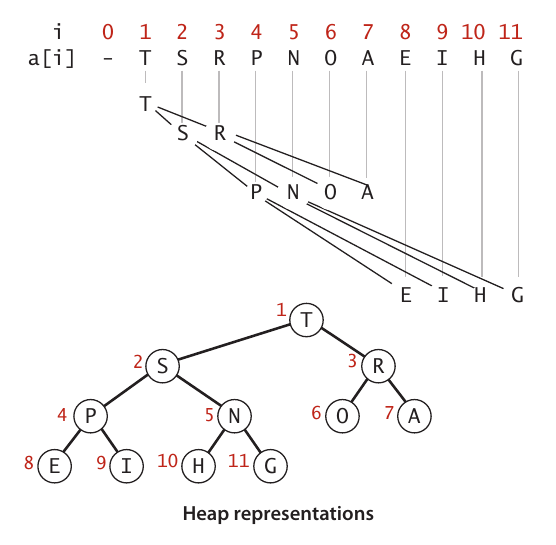
\includegraphics[width=\linewidth]{heap-representation}

		Algorithms, 4th edition, bls. 314
	\end{columns}
\end{frame}

\begin{frame}{Aðgerðir á hrúgu}
	\begin{itemize}
		\item Við þurfum að geta útfært aðgerðirnar \texttt{insert} og \texttt{delMax}
		\item Til að setja nýtt stak inn látum við það ``synda'' upp hrúguna
		\begin{itemize}
			\item Setjum það neðst í tréð
			\item Skiptum á stakinu og foreldri þess, höldum áfram þar til foreldrið er stærra
		\end{itemize}
		\item Til að fjarlægja stærsta stakið látum við stak ``sökkva'' niður hrúguna
		\begin{itemize}
			\item Afritum stærsta stakið, skiptum á staðsetningu þess og þess aftasta
			\item Fjarlægjum stærsta stakið, sem nú var aftast
			\item Skiptum á stakinu sem við settum fremst við \emph{stærra} barn sitt þar til hrúguskilyrði er aftur uppfyllt
		\end{itemize}
	\end{itemize}
\end{frame}

\headonly

\begin{frame}{Aðgerðir á hrúgu}
	\begin{center}
		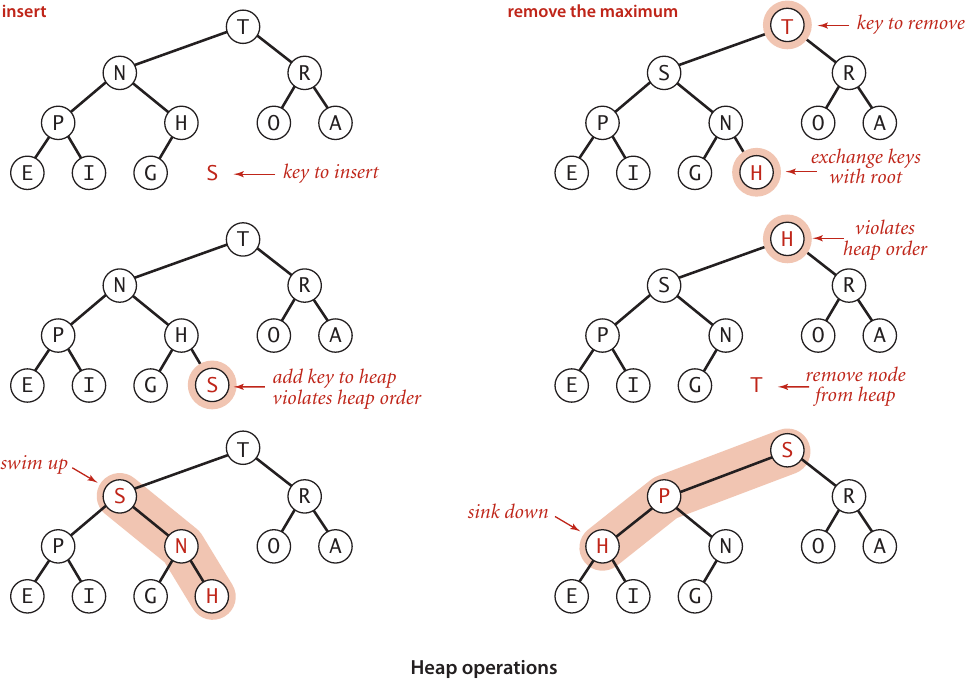
\includegraphics[width=0.8\linewidth]{heap-operations}
	\end{center}
	Algorithms, 4th edition, bls. 317
\end{frame}

\headandfoot

\begin{frame}{Útfærsla}
	\begin{columns}
		\column{0.3\textwidth}
		Algorithms, 4th edition, bls.318
		\column{0.7\textwidth}
		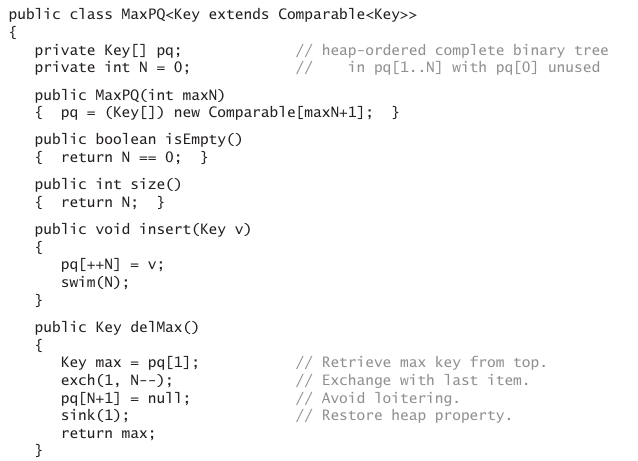
\includegraphics[width=\linewidth]{maxpq-code}
	\end{columns}
\end{frame}

\headonly

\begin{frame}[fragile]{Sink \& Swim}

		\begin{minted}[frame=lines, fontsize=\small]{java}
private void swim(int k) {
  while (k > 1 && less(k / 2, k)) {
    exch(k, k / 2);
    k = k / 2;
  }
}
		\end{minted}

		
		\begin{minted}[frame=lines, fontsize=\small]{java}
private void sink(int k) {
  while (2 * k <= n) {
    int j = 2 * k;
    if (j < n && less(j, j + 1)) j++;
    if (!less(k, j)) break;
    exch(k, j);
    k = j;
  }
}
		\end{minted}
		
\end{frame}

\headandfoot

\begin{frame}{Tími}
	\begin{itemize}
		\item Athugum - um fullskipuð tré er að ræða
		\item Innsetning og eyðing felur í sér færslu á milli hæða í trénu
		\item Fjöldi aðgerða takmarkast af hæð trésins
		      \begin{itemize}
			      \item Hæð fullskipaðs trés með $n$ hnútum er $\approx \log_2 n $
		      \end{itemize}
		\item Praktísk vandræði - langt á milli staka, hentar skyndiminni örgjörva illa
	\end{itemize}
\end{frame}

\begin{frame}{Þessi glærupakki}
	Glærurnar með gráa bakgrunnin koma frá bókarhöfundum, af \href{http://algs4.cs.princeton.edu/lectures/}{síðu bókarinnar}.

	Kóða fyrir algs4 reiknirit má finna á \url{http://algs4.cs.princeton.edu/code/}
\end{frame}

\begin{frame}{Næst}
	\begin{itemize}
		\item Nafnatöflur
		\item Helmingunarleit og tvíleitartré
		\item Lesefni: Kaflar 3.1 og 3.2 í Algorithms, 4th edition
	\end{itemize}
\end{frame}


\end{document}
